In order to state whether the the performed semantic segmentation was successful it is necessary to propose a method of assessing correctness of the resulting labelling. A trivial approach would be to present precision of a method in terms of a percentage of correctly labelled superpixels. However, this is not a very informative method as it is enough to label each superpixel with the most popular class to obtain a high score. That is why, other assessment methods are required. One of the standard ways to evaluate a given segmentation method is to use the Jaccard Index\cite{IoU}, more known as Intersection over Union (IoU). In semantic image segmentation, IoU measures the similarity between ground truth and experimental results. In order to visualise how this measure is obtained, figure \ref{fig:iou_pepper_set} was prepared. 
\begin{figure}[ht]
 \centering
  \begin{subfigure}[h]{0.32\textwidth}
    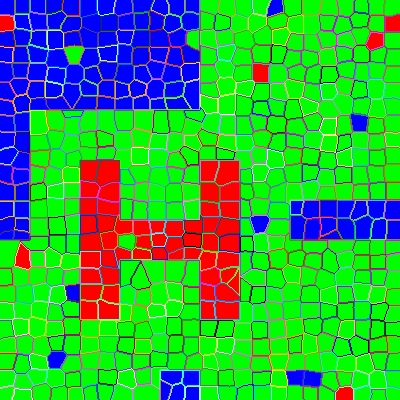
\includegraphics[width=\textwidth]{iou/image.png}
    \caption{Sample image}
    \label{fig:iou_sample_image}
  \end{subfigure}
  %
  \begin{subfigure}[h]{0.32\textwidth}
    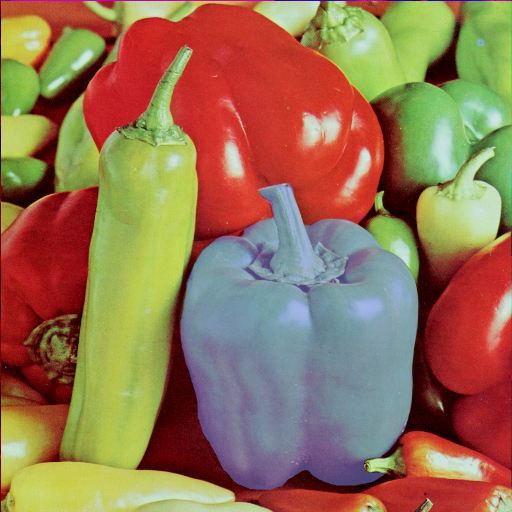
\includegraphics[width=\textwidth]{iou/reference.png}
    \caption{Ground truth}
    \label{fig:iou_reference}
  \end{subfigure}
  %
    \begin{subfigure}[h]{0.32\textwidth}
    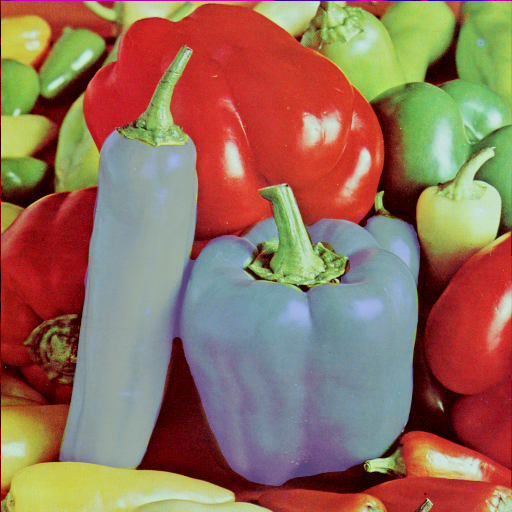
\includegraphics[width=\textwidth]{iou/experiment.png}
    \caption{Segmentation results}
    \label{fig:iou_experiment}
  \end{subfigure}
  %
  \begin{subfigure}[h]{0.32\textwidth}
    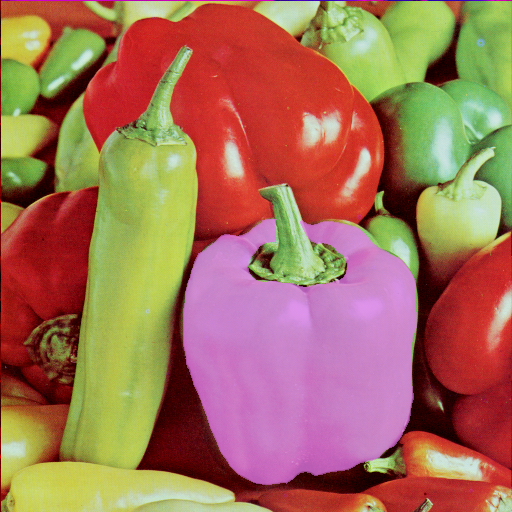
\includegraphics[width=\textwidth]{iou/intersection.png}
    \caption{Intersection}
    \label{fig:iou_intersection}
  \end{subfigure}
  %
  \begin{subfigure}[h]{0.32\textwidth}
    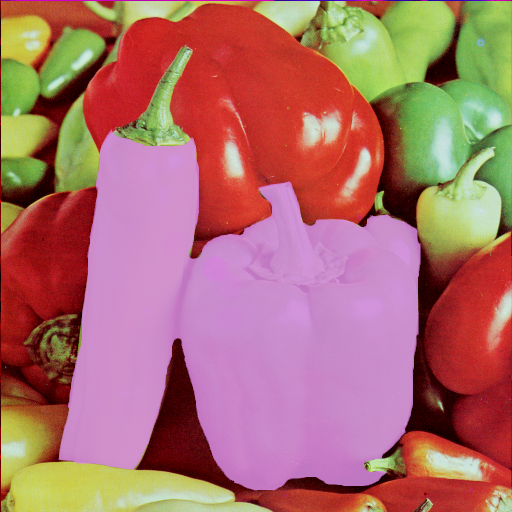
\includegraphics[width=\textwidth]{iou/union.png}
    \caption{Union}
    \label{fig:iou_union}
  \end{subfigure}
    \caption{Intersection and union of ground truth and segmentation results for a sample image needed to compute the Jaccard index}%
    \label{fig:iou_pepper_set}
\end{figure}
It shows a sample image on which semantic segmentation was performed. Ground truth is marked on a separate image as a semi-transparent blue layer. Similarly, figure \ref{fig:iou_experiment} presents the experimental results of a given segmentation method. Then, to calculate IoU two sets are needed. An intersection set, which is shown in figure \ref{fig:iou_intersection} that presents a mask of all pixels that were correctly labelled, and a union set from figure \ref{fig:iou_union}, which shows all pixels from the ground truth and from the experimental result marked together. Then, IoU can be calculated as a ratio between those two sets according to the formula \ref{eq:iou}.
\begin{equation}
    \label{eq:iou}
        IoU =\frac{\text{true positive}}{\text{true positive + false positive + false negative}} 
\end{equation}

The final evaluation of semantic segmentation results is based on an average value of IoU over all test examples and all available classes, and this metric was used to assess the precision of results in each of the performed experiments.